\section{Experimental evaluation}
We evaluate the efficiency of FlashR on statistics and machine learning
algorithms both in memory and on SSDs. We compare the R implementations of
these algorithms with the ones in two optimized parallel machine learning
libraries H$_2$O \cite{h2o} and Spark MLlib \cite{mllib}. We further use FlashR
to accelerate existing R functions in the MASS package and compare with
Revolution R Open \cite{rro}.

We conduct experiments on our local server and Amazon cloud. The local server
is a large NUMA machine with four Intel Xeon E7-4860 2.6 GHz processors,
each of which has 12 cores, 1TB of DDR3-1600 memory. The machine is equipped
with 24 OCZ Intrepid 3000 SSDs, which together are capable of 12 GB/s for read
and 10 GB/s for write. The machine runs Ubuntu 16.04 and uses ATLAS 3.10.2 as
the default BLAS library. We also run FlashR on an EC2 i3.16xlarge instance,
which has 64 virtual CPUs, 488GB of RAM and 8 NVMe SSDs. The NVMe SSDs together
provide 15.2TB of space and up to 16GB/s of sequential I/O throughput.

\subsection{Benchmark algorithms}\label{benchalg}
We benchmark FlashR with some commonly used algorithms. Like the algorithms
shown in Section \ref{sec:apps}, we implement these algorithms completely with
the R code and rely on FlashR to execute them in parallel and out of core.

\noindent \textbf{Correlation} computes pair-wise Pearson's correlation
\cite{cor} and is commonly used in statistics.

\noindent \textbf{Principal Component Analysis (PCA)} computes uncorrelated
variables from a large dataset. PCA is commonly used for dimension reduction
in many data analysis tasks. We compute PCA by computing eigenvalues on the Gramian
matrix $A^T A$ of the input matrix $A$.

\noindent \textbf{Naive Bayes} is a classifier that applies Bayes' theorem
with the ``naive'' assumption of independence between every pair of features.
Our implementation assumes data follows the normal distribution.

\noindent \textbf{Logistic regression} is a linear regression model with
categorical dependent variables. We use the LBFGS algorithm \cite{lbfgs}
to optimize logistic regression.
It converges when $logloss_{i-1}-logloss_i < 1e-6$, where $logloss_i$
is the logarithmic loss at iteration $i$.

\noindent \textbf{K-means} is an iterative clustering algorithm that
partitions data points to $k$ clusters. Its R implementation is illustrated
in Figure \ref{fig:kmeans}. In the experiments, we run k-means to split
a dataset into 10 clusters by default. It converges when no data points
move.

\noindent \textbf{Gaussian mixture models (GMM)} assumes data follows
a mixture of Gaussian distribution and learns parameters of Gaussian mixture
models from data. It typically uses the expectation-maximization (EM)
algorithm \cite{em} to fit the models, similar to k-means.

\noindent \textbf{Multivariate Normal Distribution (mvrnorm)} generates
samples from the specified multivariate normal distribution. We use
the implementation in the MASS package.

\noindent \textbf{Linear discriminant analysis (LDA)} is a linear classifier
that assumes the normal distribution with a different mean for each class
but sharing the same covariance matrix among classes. We use the implementation
in the MASS package with some trivial modifications.

%\noindent \textbf{PageRank} is a well-known algorithm for graph analysis.
%We run the R implementation in Figure \ref{pagerank} in the experiment.
%PageRank converges when
%$\forall j, abs(PR^i(v_j) - PR^{i-1}(v_{j})) < \dfrac{0.01}{n}$,
%where $PR^i(v_j)$ is the PageRank value of vertex $v_j$ at iteration $i$ and
%$n$ is the number of vertices in the graph.

\begin{table}
\begin{center}
\caption{Computation and I/O complexity of the benchmark algorithms. For
	iterative algorithms, the complexity is per iteration. $n$ is the number
	of data points, $p$ is the number of the features in a point, and $k$ is
	the number of clusters. We assume $n > p$.
}
\vspace{-10pt}
\footnotesize
\begin{tabular}{|c|c|c|c|c|}
\hline
Algorithm & Computation & I/O \\
\hline
Correlation & $O(n \times p^2)$ & $O(n \times p)$ \\
\hline
PCA & $O(n \times p^2)$ & $O(n \times p)$ \\
\hline
Naive Bayes & $O(n \times p)$ & $O(n \times p)$ \\
\hline
Logistic regression & $O(n \times p)$ & $O(n \times p)$ \\
\hline
K-means & $O(n \times p \times k)$ & $O(n \times p)$ \\
\hline
GMM & $O(n \times p^2 \times k)$ & $O(n \times p + n \times k)$ \\
\hline
mvrnorm & $O(n \times p^2)$ & $O(n \times p)$ \\
\hline
LDA & $O(n \times p^2)$ & $O(n \times p)$ \\
\hline
%PageRank & $O(nnz + n)$ & $O(nnz)$ \\
%\hline
\end{tabular}
\normalsize
\label{tbl:algs}
\end{center}
\vspace{-10pt}
\end{table}

These algorithms have various ratios of computation complexity and I/O complexity
(Table \ref{tbl:algs}) to thoroughly evaluate performance of FlashR on SSDs.
Logistic regression, K-means and GMM run iteratively and, thus, we show
their computation and I/O complexity in a single iteration.

We use two real-world datasets with billions of data points (Table \ref{tbl:data})
to benchmark the algorithms above. The Criteo dataset has over four billion data
points with binary labels (click vs. no-click), used for advertisement click
prediction \cite{criteo}. PageGraph-32ev are 32 singular vectors that we computed
on the largest connected component of a Page graph whose vertices represent Web
pages and edges represents hyperlinks between Web pages \cite{webgraph}.
To compare FlashR with other frameworks, we take part of the Criteo and
PageGraph-32ev datasets to
create smaller datasets. PageGraph-32ev-sub is the first 336 million data points
of the PageGraph-32ev dataset. Criteo-sub contains the data points collected
on the first two days, which is about one tenth of the whole dataset.

\begin{table}
\begin{center}
\caption{Datasets. All datasets are stored as dense matrices.}
\vspace{-10pt}
\footnotesize
\begin{tabular}{|c|c|c|c|c|}
\hline
Data Matrix & \#rows & \#cols \\
\hline
PageGraph-32ev \cite{webgraph} & 3.5B & 32 \\
\hline
Criteo \cite{criteo} & 4.3B & 40 \\
\hline
PageGraph-32ev-sub \cite{webgraph} & 336M & 32 \\
\hline
Criteo-sub \cite{criteo} & 325M & 40 \\
\hline
\end{tabular}
\normalsize
\label{tbl:data}
\end{center}
\vspace{-10pt}
\end{table}

%\vspace{-8pt}
\subsection{Comparative performance}
%\vspace{-4pt}
We evaluate FlashR against H$_2$O \cite{h2o} and Spark MLlib \cite{mllib} as well
as Revolution R Open \cite{rro} in our local server and in the Amazon
cloud. When running in the 48 CPU core local server, all frameworks
use 48 threads and H$_2$O and MLlib have a large heap size (500GB) to ensure that
all data are cached in memory. When running in the cloud, we run FlashR
in an i3.16xlarge instance
and MLlib in a cluster of four EC2 m4.16xlarge instances (256 CPU cores, 1TB RAM
and 20Gbps network). We also use FlashR to parallelize functions (mvrnorm and LDA)
in the R MASS package and compare their speed with Revolution R Open. We use
Spark v2.0.1, H$_2$O v3.14.2 and Revolution R Open v3.3.2.

\begin{figure}
  \vspace{-5pt}
	\centering
	\footnotesize
	\begin{subfigure}{.5\textwidth}
		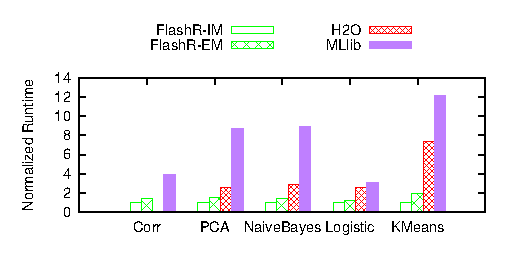
\includegraphics{FlashMatrix_figs/FlashR-vs-dist.eps}
		\caption{In a large parallel machine with 48 CPU cores.}
		\label{perf:para}
	\end{subfigure}

	\vspace{3pt}
	\begin{subfigure}{.5\textwidth}
		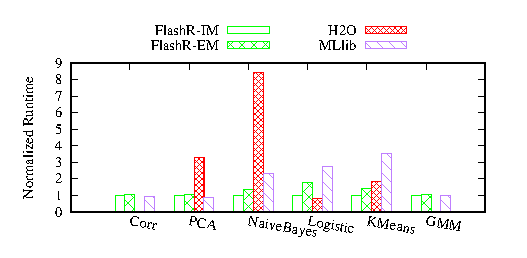
\includegraphics{FlashMatrix_figs/FlashR-vs-dist-EC2.eps}
		\caption{In the Amazon cloud. FlashR-IM and FlashR-EM run on one
			EC2 i3.16xlarge instance (64 CPU cores) and Spark MLlib runs
		on a cluster of four EC2 m4.16xlarge instances (256 CPU cores).}
		\label{perf:cloud}
	\end{subfigure}
	\vspace{-8pt}
	\caption{The normalized runtime of FlashR in memory (FlashR-IM) and
	on SSDs (FlashR-EM) compared with H$_2$O and Spark MLlib. Correlation and GMM
	are not available in H$_2$O. We run k-means and GMM on the PageGraph-32ev-sub
	dataset and all other algorithms on the Criteo-sub dataset.}
	\label{perf:rt}
  \vspace{-10pt}
\end{figure}

FlashR outperforms H$_2$O and Spark MLlib significantly on all algorithms
(Figure \ref{perf:para}) in the large parallel machine with 48 CPU cores.
When all frameworks run on the same hardware, FlashR in memory (FlashR-IM)
achieves 4 to 10 times performance gain when compared
with MLlib, and 3 to 20 times performance gain when compared with H$_2$O.
When running on SSDs, FlashR achieves at least half the speed of running in
memory. All implementations rely on BLAS for matrix multiplication. H$_2$O
and MLlib have to implement non-BLAS operations with Java and Scala,
respectively. Spark also materializes operations such as aggregation
separately. In contrast,
FlashR fuses matrix operations and performs two-level partitioning to
minimize data movement in the memory hierarchy and keeps data in local
memory to achieve high memory bandwidth.

We further evaluate the speed of FlashR on Amazon EC2 cloud and compare it with
Spark MLlib on an EC2 cluster (Figure \ref{perf:cloud}). H$_2$O recommends
allocating a total of four times the memory of the input data. As such,
4 m4.16xlarge instances provide sufficient memory and computation power to
Spark MLlib and H$_2$O to process the datasets (PageGraph-32ev-sub and Criteo-sub).
Even though Spark MLlib and H$_2$O have four times as much computation power as FlashR,
FlashR still outperforms both distributed machine learning libraries in most algorithms.
Because the NVMes in i3.16xlarge provide higher I/O throughput than the SSDs
in our local server, the performance gap between FlashR-IM and FlashR-EM is
smaller.

\begin{figure}[b]
  \vspace{-10pt}
	\begin{center}
		\footnotesize
		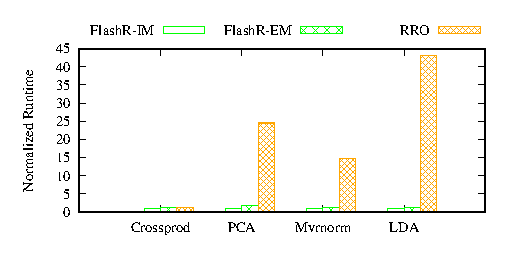
\includegraphics{FlashMatrix_figs/FlashR-vs-RRO.eps}
		\vspace{-10pt}
		\caption{In-memory (FlashR-IM) and out-of-fore (FlashR-EM) FlashR
		compared with Revolution R Open on a data matrix with one million rows
		and one thousand columns when running on the parallel machine with
		48 CPU cores.}
		\label{fig:fmR}
	\end{center}
  \vspace{-15pt}
\end{figure}

FlashR running both in memory and on SSDs outperforms Revolution R Open by more
than an order of magnitude even on a small dataset ($n=1,000,000$ and $p=1000$)
(Figure \ref{fig:fmR}).
Revolution R Open uses Intel MKL to parallelize matrix multiplication. As such,
we only compare the two frameworks with computations that use matrix
multiplication heavily. Both FlashR and Revolution R Open run the mvrnorm
and LDA implementations from the MASS package. For simple matrix operations such as crossprod,
FlashR slightly outperforms Revolution R Open. For more complex computations,
the speed gap between FlashR and Revolution R increases. Even though matrix multiplication
is the most computation-intensive operation in an algorithm, it is insufficient
to only parallelize matrix multiplication to achieve high efficiency.

\subsection{Scalability}

We show the scalability of FlashR on the billion-scale datasets in Table
\ref{tbl:data}. In these experiments, we run the iterative algorithms on
the datasets until they converge (see their convergence condition in Section
\ref{benchalg}).

\begin{table}
\begin{center}
	\caption{The runtime and memory consumption of FlashR on the billion-scale
		datasets on the 48 CPU core machine. The runtime of iterative
		algorithms is measured when the algorithms converge. We run k-means
		on PageGraph-32ev and the remaining algorithms on Criteo.}
\vspace{-10pt}
\footnotesize
\begin{tabular}{|c|c|c|}
\hline
	& Runtime (min) & Peak memory (GB) \\
\hline
Correlation & $1.5$ & $1.5$ \\
\hline
PCA & $2.3$ & $1.5$ \\
\hline
NaiveBayes & $1.3$ & $3$ \\
\hline
LDA & $38$ & $8$ \\
\hline
% in 23 iterations.
Logistic regression & $29.8$ & $26$ \\
\hline
k-means & $18.5$ & $28$ \\
\hline
GMM & $350.6$ & $18$ \\
\hline
\end{tabular}
\normalsize
\label{tbl:scale}
\end{center}
\vspace{-10pt}
\end{table}

Even though we process the billion-scale datasets in a single machine, none of
the algorithms are prohibitively expensive. Simple algorithms, such as
Naive Bayes and PCA, require one or two passes over the datasets and take
only one or two minutes to complete. Logistic regression and k-means take
about $10-20$ iterations to converge.
Nevertheless, all of the iterative algorithms take about one hour or less.

FlashR scales to datasets with billions of data points easily when running
out of core. All of the algorithms have negligible memory consumption.
The scalability of FlashR is mainly bound by the capacity of SSDs.
The functional programming
interface generates a new matrix in each matrix operation, which potentially
leads to high memory consumption. Thanks to lazy evaluation and virtual matrices,
FlashR only needs to materialize the small matrices to effectively reduce
memory consumption.
%Owing to lazy evaluation, FlashR does not store majority of matrices in
% the computation physically. As such, its in-memory 
%out-of-core execution barely increases memory consumption from
%the minimum memory requirement of the algorithms. 
%This indicates that the out-of-core execution consumes small space on SSDs, which leads to
%very high scalability.

%\vspace{-8pt}
\subsection{Computation complexity versus I/O complexity}
%\vspace{-4pt}
We further compare the speed of FlashR in memory and in external memory
for algorithms with different computation and I/O complexities.
We pick three algorithms from Table \ref{tbl:algs}: \textit{(i)} Naive Bayes,
whose computation and I/O complexity are the same, \textit{(ii)}
correlation, whose computation complexity grows quadratically with $p$ while
its I/O complexity grows linearly with $p$, \textit{(iii)} k-means, whose computation
complexity grows linearly with $k$ while its I/O complexity is independent
from $k$. We run the first two algorithms on datasets with $n=100M$ and $p$
varying from 8 to 512. We run k-means on a dataset with $p=100M$ and $p=32$
and vary the number of clusters from 2 to 64.

\begin{figure}[t]
	\begin{center}
		\footnotesize
		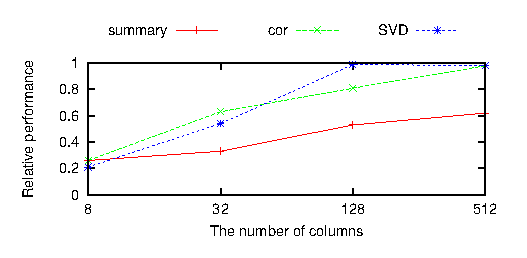
\includegraphics{FlashMatrix_figs/IM-vs-EM-stat.eps}
		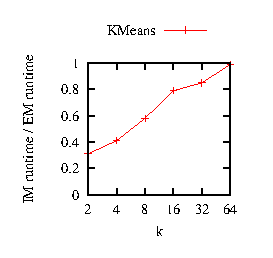
\includegraphics{FlashMatrix_figs/IM-vs-EM-clust.eps}
		\vspace{-10pt}
		\caption{The relative runtime of FlashR in memory versus on SSDs
		on a dataset with $n=100M$ while varying $p$ (the number of features)
		on the left and varying $k$ (the number of clusters) on the right.}
		\label{perf:stat}
	\end{center}
  \vspace{-15pt}
\end{figure}

As the number of features or clusters increases, the performance gap between
in-memory and external-memory execution narrows and the external-memory
performance approaches in-memory performance for correlation and k-means
but not Naive Bayes (Figure \ref{perf:stat}). This observation conforms with
the computation and I/O complexity of the algorithms in Table \ref{tbl:algs}.
For correlation and k-means, the number of clusters or features causes computation
to grow more quickly than the I/O, driving performance toward a computation bound.
% When the number of features
%gets larger, the computation of matrix multiplication in
%correlation and SVD grows more rapidly than I/O and eventually CPU becomes
%the bottleneck. The current implementation of correlation requires an additional
%pass on the input matrix to compute column-wise mean values, which results in
%lower external-memory performance. Similarly, as the number of clusters
%increases, the computation of k-means and GMM increases rapidly and
%these algorithms are dominated by their CPU computation as the number
%of clusters gets larger. 
The computation bound can be realized on few features or clusters for an I/O throughput of 10GB/s.
Because most of the machine learning algorithms in Table \ref{tbl:algs} have
computation complexities that grow quadratically with $p$, we expect FlashR on SSDs to
achieve the same speed as in memory on datasets with a higher dimension size.

%\begin{figure}
%	\begin{center}
%		\footnotesize
%		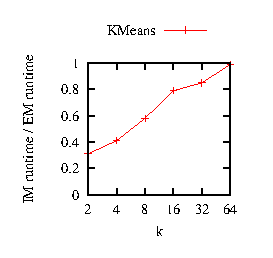
\includegraphics{FlashMatrix_figs/IM-vs-EM-clust.eps}
%		\caption{{\em Clustering} scaleup: FlashMatrix performance on SSDs 
%      normalized to in-memory performance as the number of clusters vary. 
%%      KMeans operates on the \rb{Friendster32} matrix and GMM on the  
%%			by its performance in memory. As the number of clusters increases,
%%			the external-memory performance of these implementations approach
%%			to their in-memory performance.}
%}
%		\label{perf:clust}
%	\end{center}
%\end{figure}

\subsection{Effectiveness of optimizations}
We illustrate the effectiveness of our memory optimizations in FlashR.
We focus on two main optimizations: matrix operation fusion in main memory
to reduce data movement between SSDs and main memory (mem-fuse), and matrix
operation fusion in CPU cache to reduce data movement between main memory and
CPU cache (cache-fuse).

Both optimizations have significant performance improvement on all
algorithms when FlashR runs on SSDs (Figure \ref{perf:em_opts}).
Operation fusion in main memory (mem-fuse) achieves
substantial performance improvement in most algorithms, even in GMM,
which has the highest asymptotic computation complexity. 
%Even though the SSDs deliver an I/O throughput of 10GB/s, 
Materializing every matrix operation
separately causes SSDs to be the main bottleneck in the system and
fusing matrix operations in memory significantly reduces I/O.
% and improves performance by a large factor. 
Operation fusion in the CPU cache (cache-fuse) doubles or even triples
performance in some of the algorithms,
which suggests that memory bandwidth is a limiting performance factor once 
I/O has been optimized.
 %This suggests that with sufficient 
%I/O optimizations, many machine learning algorithms that run on fast SSDs can be bottlenecked by
%the bandwidth of main memory, instead of I/O. 
%Even though it is less noticeable,
%Finally, reducing large memory allocation (mem-alloc) improves I/O performance and almost doubles
%the overall performance of all algorithms.

\begin{figure}
	\begin{center}
		\footnotesize
		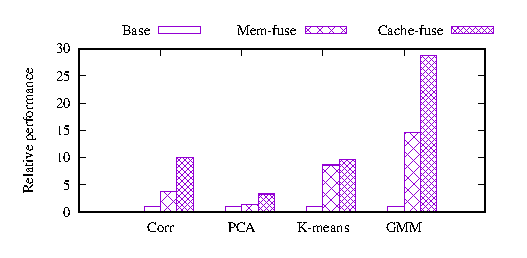
\includegraphics{FlashMatrix_figs/opts-EM.eps}
		\vspace{-10pt}
		\caption{The effectiveness of optimizations on different algorithms
		running on SSDs. The optimizations are applied to FlashR
		incrementally.}
		\label{perf:em_opts}
	\end{center}
\end{figure}
